\documentclass[
	12pt,
	a4paper,
	ngerman,
	openright,
	final,
	listof=nochaptergap,
	]{scrbook}
\usepackage{cmap}
\usepackage[T1]{fontenc}
\usepackage[utf8]{inputenc}

% ##################################################
% Unterstuetzung fuer die deutsche Sprache
% ##################################################
%\usepackage{ngerman}
\usepackage[ngerman]{babel}
\usepackage{graphicx}
\usepackage{wrapfig}
\usepackage{textcomp}
\usepackage{xspace}
\usepackage{amssymb}
\usepackage{savesym}
\savesymbol{checkmark}
\usepackage{dingbat}
\usepackage{booktabs}
\usepackage{lscape}

\usepackage{array,ragged2e}

\newcolumntype{P}[1]{>{\RaggedRight\arraybackslash}p{#1}}
\newcolumntype{C}[1]{>{\centering\arraybackslash}p{#1}}

% ##################################################
% Dokumentvariablen
% ##################################################

% Persoenliche Daten
\newcommand{\docNachname}{Petrov}
\newcommand{\docVorname}{Anton}


% Dokumentdaten
\newcommand{\docTitle}{Aktuelle Trends Im Compilerbau}
\newcommand{\docUntertitle}{} % Kein Untertitel
%\newcommand{\docUntertitle}{UNTERTITEL}
% Arten der Arbeit: Bachelorthesis, Masterthesis, Seminararbeit, Diplomarbeit
\newcommand{\docArtDerArbeit}{Forschungsprojekt}
%Studiengaenge: Allgemeine Informatik Bachelor, Computer Networking Bachelor,
% Software-Produktmanagement Bachelor, Advanced Computer Scinece Master
\newcommand{\docStudiengang}{Informatik Master}
\newcommand{\docAbgabedatum}{14.07.2022}
\newcommand{\docErsterReferent}{Prof. Dr. Hollunder}

% ##################################################
% Allgemeine Pakete
% ##################################################

% Abbildungen einbinden
\usepackage{graphicx}

% Zusaetsliche Sonderzeichen
\usepackage{dingbat}

% Symbole Haken und X [OPTIONAL]
%\usepackage{pifont}
%\newcommand{\cmark}{\ding{51}}
%\newcommand{\xmark}{\ding{55}}

% Farben
\usepackage{color}
\usepackage[usenames,dvipsnames,svgnames,table]{xcolor}

% Maskierung von URLs und Dateipfaden
\usepackage[hyphens]{url}

% Deutsche Anfuehrungszeichen
\usepackage[babel, german=quotes]{csquotes}

% Pakte zur Index-Erstellung (Schlagwortverzeichnis)
\usepackage{index}
\makeindex

% Ipsum Lorem
% Paket wird nur für das Beispiel gebraucht und kann gelöscht werden
\usepackage{lipsum}

% ##################################################
% Seitenformatierung
% ##################################################
\usepackage[
	portrait,
	bindingoffset=1.5cm,
	inner=2.5cm,
	outer=2.5cm,
	top=3cm,
	bottom=2cm,
	%showframe, %Aktivieren um Seitengrenzen anzuzeigen
	%includeheadfoot
	]{geometry}

% ##################################################
% Kopf- und Fusszeile
% ##################################################

\usepackage{fancyhdr}

\pagestyle{fancy}
\fancyhf{}
\fancyhead[EL,OR]{\sffamily\thepage}
\fancyhead[ER,OL]{\sffamily\nouppercase{\leftmark}}

\fancypagestyle{headings}{}

\fancypagestyle{plain}{}

\fancypagestyle{empty}{
	\fancyhf{}
	\renewcommand{\headrulewidth}{0pt}
}

%Speichert \chaptermark in \oldchaptermark damit 
% es für die Anhänge zurückgesetzt werden kann
\let\oldchaptermark\chaptermark

%Kein "Kapitel # NAME" in der Kopfzeile
\renewcommand{\chaptermark}[1]{
	\markboth{#1}{}
   	\markboth{\thechapter.\ #1}{}
}

\let\OldTexttrademark\texttrademark
\renewcommand{\texttrademark}{\OldTexttrademark\xspace}%

% ##################################################
% Schriften
% ##################################################

% Stdandardschrift festlegen
\renewcommand{\familydefault}{\sfdefault}

% Standard Zeilenabstand: 1,5 zeilig
\usepackage{setspace}
\onehalfspacing 

% Schriftgroessen festlegen
\addtokomafont{chapter}{\sffamily\large\bfseries} 
\addtokomafont{section}{\sffamily\normalsize\bfseries} 
\addtokomafont{subsection}{\sffamily\normalsize\mdseries} 
\addtokomafont{subsubsection}{\sffamily\normalsize\mdseries} 
\addtokomafont{caption}{\sffamily\normalsize\mdseries} 

%Einrücken von Absätzen deaktivieren
\setlength{\parindent}{0pt}

%Zeilenabstand bei abstätzen
%\usepackage{parskip}

% ##################################################
% Inhaltsverzeichnis / Allgemeine Verzeichniseinstellungen
% ##################################################

\usepackage{tocloft}

% Punkte auch bei Kapiteln
\renewcommand{\cftchapdotsep}{3}
\renewcommand{\cftdotsep}{3}

% Schriftart und -groesse im Inhaltsverzeichnis anpassen
\renewcommand{\cftchapfont}{\sffamily\normalsize}
\renewcommand{\cftsecfont}{\sffamily\normalsize}
\renewcommand{\cftsubsecfont}{\sffamily\normalsize}
\renewcommand{\cftchappagefont}{\sffamily\normalsize}
\renewcommand{\cftsecpagefont}{\sffamily\normalsize}
\renewcommand{\cftsubsecpagefont}{\sffamily\normalsize}

%Zeilenabstand in den Verzeichnissen einstellen
\setlength{\cftparskip}{.5\baselineskip}
\setlength{\cftbeforechapskip}{.1\baselineskip}

%Einrücken von Absätzen deaktivieren
%\setlength{\parindent}{0pt}

%Zeilenabstand bei abstätzen
\usepackage{parskip}

% ##################################################
% Abbildungsverzeichnis und Abbildungen
% ##################################################

\usepackage{caption}

\usepackage{wrapfig}

% Nummerierung von Abbildungen
\renewcommand{\thefigure}{\arabic{figure}}
\usepackage{chngcntr}
\counterwithout{figure}{chapter}

% Abbildungsverzeichnis anpassen
\renewcommand{\cftfigpresnum}{Abbildung }
\renewcommand{\cftfigaftersnum}{:}

% Breite des Nummerierungsbereiches [Abbildung 1:]
\newlength{\figureLength}
\settowidth{\figureLength}{\bfseries\cftfigpresnum\cftfigaftersnum}
\addtolength{\figureLength}{2mm} %extra offset
\setlength{\cftfignumwidth}{\figureLength}
\setlength{\cftfigindent}{0cm}

% Schriftart anpassen
\renewcommand\cftfigfont{\sffamily}
\renewcommand\cftfigpagefont{\sffamily}

%standardpfad anpassen
\graphicspath{ {../src/content/pictures/} }

% ##################################################
% Tabellenverzeichnis und Tabellen
% ##################################################

% Nummerierung von Tabellen
\renewcommand{\thetable}{\arabic{table}}
\counterwithout{table}{chapter}

% Tabellenverzeichnis anpassen
\renewcommand{\cfttabpresnum}{Tabelle }
\renewcommand{\cfttabaftersnum}{:}

% Breite des Nummerierungsbereiches [Abbildung 1:]
\newlength{\tableLength}
\settowidth{\tableLength}{\bfseries\cfttabpresnum\cfttabaftersnum}
\addtolength{\tableLength}{3mm} %extra offset
\setlength{\cfttabnumwidth}{\tableLength}
\setlength{\cfttabindent}{0cm}

%Schriftart anpassen
\renewcommand\cfttabfont{\sffamily}
\renewcommand\cfttabpagefont{\sffamily}

% Unterdrueckung von vertikalen Linien
\usepackage{booktabs}

%Multi row für spezifische zellen
\usepackage{multirow}

%Additional table package
\usepackage{tabu}

% ##################################################
% Listings (Quellcode)
% ##################################################

\usepackage{listings}

%use typewriter font which supports bold characters
\usepackage{beramono}

\definecolor{codegreen}{rgb}{0,0.6,0}
\definecolor{codegray}{rgb}{0.5,0.5,0.5}
\definecolor{codepurple}{rgb}{0.5,0,0.33}
\definecolor{codepurblue}{rgb}{0.16,0.0,1.0}
\definecolor{backcolour}{rgb}{0.95,0.95,0.92}

\lstdefinestyle{codestyle}{
    backgroundcolor=\color{backcolour},   
    commentstyle=\color{codegreen},
    keywordstyle=\bfseries\color{codepurple},
    numberstyle=\tiny\color{codegray},
    stringstyle=\color{codepurblue},
    basicstyle=\scriptsize\ttfamily,
    breakatwhitespace=false,         
    breaklines=true,                 
    captionpos=b,                    
    keepspaces=true,                 
    numbers=left,                     
    numbersep=5pt,                 
    showspaces=false,                
    showstringspaces=false,
    showtabs=false,                  
    tabsize=2
}

\lstset{style=codestyle}

%Code auschnitt importieren aus datei
%\mylisting{from}{to}{language}{file}{descr}{path}
\newcommand{\mylisting}[6]{
\lstinputlisting[language=#3,
				firstnumber=#1,
				firstline=#1,
				lastline=#2,
				caption={#4, #5}, 
				label={implementation_listing_#4_#5}]
				{#6}
}

% ##################################################
% Appendix
% ##################################################

%Calc packet für berechnungen
\usepackage{calc}

%Appendix paket, setzen der flags für das TOC
\usepackage[title,titletoc]{appendix} 

%Umbenennen der überschrift für die Anhänge 
\renewcommand{\appendixtocname}{Anhänge}

%Befehl für einen neuen Bericht und die erste seite als bild
\newcommand{\appendixsection}[2]{
\section{#1}
\appendixsingle{#2}
}

%Befehl für einzelne seite als bild eingefasst, damit überschrift und kopfzeile
% bestehen bleibt. 
\newcommand{\appendixsingle}[1]{
\vspace{-10cm}
\vfill
\mbox{}\hspace{-1.5cm}\includegraphics[width=\linewidth+3cm]{#1}\hspace{-1.5cm}\mbox{}
\vspace{-10cm}
\vfill
\mbox{}
}

% appendix chapter
\newcommand{\appendixchapter}[1]{
	\cleardoublepage
	\pagenumbering{arabic}
	\renewcommand{\thepage}{\thechapter-\arabic{page}}
	\chapter{#1}
}

% insert monthly report pdf as picture in order to keep page header
\newcommand{\monthlyreport}[2]{
	\section{#1}
	\centering
	\includegraphics[trim=55 35 55 35,clip,width=1\textwidth]{#2}
	\clearpage
}

%Datenträger Tabelle
\definecolor{lightgray}{gray}{0.85}
\definecolor{ultralightgray}{gray}{0.95}
\definecolor{mygray}{gray}{0.70}

% ##################################################
% Theoreme
% ##################################################
  	
% Umgebung fuer Beispiele
\newtheorem{beispiel}{Beispiel}

% Umgebung fuer These
\newtheorem{these}{These}

% Umgebung fuer Definitionen
\newtheorem{definition}{Definition}
  	
% ##################################################
% Literaturverzeichnis
% ##################################################

\usepackage[backend=biber,citestyle=ieee,urldate=long, dateabbrev=false]{biblatex}
\addbibresource{bibtex.bib}
\setlength\bibitemsep{.5\baselineskip}
\setcounter{biburlnumpenalty}{9000} % break URLs on numbers
\setcounter{biburllcpenalty}{9000}  % break URLs on lower case letters
\setcounter{biburlucpenalty}{9000}  % break URLs on upper case letters

\usepackage[hyphenbreaks]{breakurl}
\usepackage[hyphens]{url}

% ##################################################
% Abkuerzungsverzeichnis
% ##################################################

\usepackage[printonlyused]{acronym}

% ##################################################
% PDF / Dokumenteninternelinks
% ##################################################

\usepackage[
	colorlinks=false,
   	linkcolor=black,
   	citecolor=black,
  	filecolor=black,
	urlcolor=black,
    bookmarks=true,
    bookmarksopen=true,
    bookmarksopenlevel=3,
    bookmarksnumbered,
    plainpages=false,
    pdfpagelabels=true,
    hyperfootnotes,
    pdftitle ={\docTitle},
    pdfauthor={\docVorname~\docNachname},
    pdfcreator={\docVorname~\docNachname}]{hyperref}
\usepackage[noabbrev]{cleveref}

% ####################################################
% Command für einfache QUellenangabe bei Bilder, etc.
% ####################################################

\newcommand{\source}[1]{
	\caption*{Quelle: {#1}} }

\newcommand*{\captionsource}[2]{%
	\caption[{#1}]{%
		#1%
		{} #2%
	}%
}

\newcommand{\R}{$^{\circledR}$}
\newcommand{\estimates}{\mathrel{\hat{=}}}
\usepackage{longtable}



%\RedeclareSectionCommand[beforeskip=1\baselineskip,afterskip=0.5\baselineskip]{section}
%\RedeclareSectionCommand[beforeskip=1\baselineskip,afterskip=0.5\baselineskip]{subsection}

%DIF PREAMBLE EXTENSION ADDED BY LATEXDIFF
%DIF UNDERLINE PREAMBLE %DIF PREAMBLE
\RequirePackage[normalem]{ulem} %DIF PREAMBLE
\RequirePackage{color}\definecolor{RED}{rgb}{1,0,0}\definecolor{BLUE}{rgb}{0,0,1} %DIF PREAMBLE
\providecommand{\DIFadd}[1]{{\protect\color{blue}\uwave{#1}}} %DIF PREAMBLE
\providecommand{\DIFdel}[1]{{\protect\color{red}\sout{#1}}}                      %DIF PREAMBLE
%DIF SAFE PREAMBLE %DIF PREAMBLE
\providecommand{\DIFaddbegin}{} %DIF PREAMBLE
\providecommand{\DIFaddend}{} %DIF PREAMBLE
\providecommand{\DIFdelbegin}{} %DIF PREAMBLE
\providecommand{\DIFdelend}{} %DIF PREAMBLE
%DIF FLOATSAFE PREAMBLE %DIF PREAMBLE
\providecommand{\DIFaddFL}[1]{\DIFadd{#1}} %DIF PREAMBLE
\providecommand{\DIFdelFL}[1]{\DIFdel{#1}} %DIF PREAMBLE
\providecommand{\DIFaddbeginFL}{} %DIF PREAMBLE
\providecommand{\DIFaddendFL}{} %DIF PREAMBLE
\providecommand{\DIFdelbeginFL}{} %DIF PREAMBLE
\providecommand{\DIFdelendFL}{} %DIF PREAMBLE
%DIF END PREAMBLE EXTENSION ADDED BY LATEXDIFF


\begin{document}

\setcounter{secnumdepth}{3}

% Titelblatt
\begin{titlepage}
\pagestyle{empty}

% ##################################################
% HFU-Logo einbinden
% ##################################################
\begin{flushright}
\begin{figure}[ht]
\flushright

\includegraphics[height=3cm]{content/pictures/hfu.jpg}
\end{figure}
\end{flushright}

% ##################################################
% Titel
% ##################################################
\begin{center}
{\fontsize{18}{22} \selectfont \docArtDerArbeit}\\[5mm]
{\fontsize{18}{22} \selectfont im Studiengang} \\[5mm]
{\fontsize{18}{22} \selectfont \docStudiengang}\\
\vspace{1cm}
\begin{onehalfspace}
{\fontsize{22}{26} \selectfont \textbf{\docTitle}}\\[5mm]
{\fontsize{18}{22} \selectfont \docUntertitle}


\end{onehalfspace}

%
\includegraphics[height=7cm]{content/pictures/WhileLang.pdf}
\end{center}

% ##################################################
% Zusatzinformationen
% ##################################################
\vfill
\begin{center}
\begin{tabular}{lcl}
Referent  		&:& \docErsterReferent 	\\ \\
Vorgelegt am 	&:& \docAbgabedatum 	\\ \\
Vorgelegt von 	&:& Anton Petrov\\& &Richard Hempel
\end{tabular}
\end{center}
\end{titlepage}

\cleardoubleemptypage

\frontmatter
\pagenumbering{Roman}
  

% Abstract
\chapter*{Abstract}\markboth{Abstract}{}
\addcontentsline{toc}{chapter}{Abstract}

Compiler und Programmiersprachen sind das tägliche Werkzeug von vielen Programmierern, doch scheinen nur wenige ein Verständnis dafür zu haben, was eine Programmiersprache genau ist und welche Schritte ein Compiler durchläuft, bis ein ausführbares Programm erzeugt wird. In der vorliegenden Arbeit werden die Bestandteile einer Programmiersprache und eines Compilers vorgestellt und Schritt für Schritt erläutert, indem eine Programmiersprache samt dazugehörigem Compiler entwickelt wird. Ebenfalls wird erläutert, wie die neue Programmiersprache in die IDE \enquote{Visual Studio Code} eingebunden wurde.

Zunächst wird eine Grammatik für die Sprache definiert und anschließend mit dem Parsergenerator \enquote{ANTLR} ein dazugehöriger Lexer und Parser erzeugt, um sie im Compiler und in der IDE-Erweiterung zu nutzen. Anschließend wird der Nutzen der semantischen Analyse erläutert und erklärt, wie sie für die Sprache implementiert wurde. Im nächsten Schritt wird die Erzeugung von Javabytecode mithilfe der Bibliothek ASM vorgestellt.

Das Ergebnis ist eine funktionstüchtige Programmiersprache mit einem einsatzfähigen Compiler und hilfreicher IDE-Integration, welche zur Lehre im Modul \enquote{Automaten Und Formale Sprachen} eingesetzt werden könnte.
\cleardoubleemptypage


% Inhaltsverzeichnis
\phantomsection
\addcontentsline{toc}{chapter}{Inhaltsverzeichnis}
\tableofcontents
\cleardoubleemptypage

% Abbildungsverzeichnis einbinden und ins Inhaltsverzeichnis
% WORKAROUND: tocloft und KOMA funktionieren zusammen nicht
% korrekt\phantomsection
\phantomsection 
\addcontentsline{toc}{chapter}{\listfigurename} 
\listoffigures
\cleardoubleemptypage

% Tabellenverzeichnis einbinden und ins Inhaltsverzeichnis
% WORKAROUND: tocloft und KOMA funktionieren zusammen nicht
% korrekt\phantomsection
\phantomsection
\addcontentsline{toc}{chapter}{\listtablename}
\listoftables
\cleardoubleemptypage

% Quellcodeverzeichnis einbinden und ins Inhaltsverzeichnis
\phantomsection
\addcontentsline{toc}{chapter}{Quellcodeverzeichnis}

%Define listing
\makeatletter
\begingroup\let\newcounter\@gobble\let\setcounter\@gobbletwo
\globaldefs\@ne \let\c@loldepth\@ne
\newlistof{listings}{lol}{\lstlistlistingname}
\endgroup
\let\l@lstlisting\l@listings
\makeatother
\setlength{\cftlistingsindent}{0em}
\renewcommand{\cftlistingsafterpnum}{\vskip0pt} %Spacing between entries
\renewcommand*{\cftlistingspresnum}{\lstlistingname~}
\settowidth{\cftlistingsnumwidth}{\cftlistingspresnum}
\renewcommand{\lstlistlistingname}{Quellcodeverzeichnis}
% Tabellenverzeichnis anpassen
\renewcommand{\lstlistingname}{Codeauschnitt}
\renewcommand{\cftlistingsaftersnum}{:}
% Breite des Nummerierungsbereiches [Codeauschnitt 1:]
\newlength{\codeLength}
\settowidth{\codeLength}{\bfseries\lstlistingname\cftlistingsaftersnum}
\addtolength{\codeLength}{5mm}
\setlength{\cftlistingsnumwidth}{\codeLength}
\lstlistoflistings
\cleardoubleemptypage

% Abkürzungsverzeichnis
\chapter*{Abkürzungsverzeichnis}\markboth{Abkürzungsverzeichnis}{}
\addcontentsline{toc}{chapter}{Abkürzungsverzeichnis}

\begin{acronym}[LoRaWAN]

\acro{asf}[ASF]{Advanced Software Framework}

\acro{css}[CSS]{Chirp Spread Spectrum}
\acro{csv}[CSV]{Comma-Separated-Values}
	
\acro{edbg}[EDBG]{Embedded Debugger}

\acro{ffd}[FFD]{Full Function Device}
\acro{fsm}[FSM]{Finite State Machine}

\acro{iot}[IoT]{Internet Of Things}
\acro{io}[IO]{Input/Output}
\acro{ism}[ISM]{Industrial Scientific and Medical}
\acro{isr}[ISR]{Interrupt Service Routine}

\acro{lns}[LNS]{LoRaWAN Network Server}
\acro{lorawan}[LoRaWAN]{Long Range Wide Area Network}
\acro{lpwan}[LPWAN]{Low-Power, Wide Area Network}
\acroplural{lpwan}[LPWAN]{Low-Power, Wide Area Networks}

\acro{mac}[MAC]{Media Access Control}
\acro{mit}[MIT]{Massachusetts Institute of Technology}
\acro{miwi}[MiWi]{Microchip Wireless}
\acro{mtce}[MTCE]{MinebeaMitsumi Technology Center Europe GmbH}

\acro{p2p}[P2P]{Peer To Peer}
\acro{pan}[PAN]{Personal Area Network}
\acro{phy}[PHY]{Physical}

\acro{rfd}[RFD]{Reduced Function Device}
\acro{rssi}[RSSI]{Received Signal Strength Indication}
\acro{rx}[Rx]{Receive}

\acro{sf}[SF]{Spreading Factor} % Groß = Große Reichweite
\acro{sip}[SiP]{System-in-Package}

\acro{teg}[TEG]{Thermoelektrischer Generator}
\acro{toa}[TOA]{Time On Air}
\acro{ttn}[TTN]{The Things Network}
\acro{tx}[Tx]{Transmision}

\acro{uart}[UART]{Universal Asynchronous Receiver Transmitter}

\acro{wpan}[WPAN]{Wireless Personal Area Network}

\end{acronym}


\mainmatter

\chapter{Einleitung}


\section{Motivation}
Dieses Unterkapitel steht in seiner eigenen Datei

\section{Zielsetzung}
Funktionsweise eines Compilers //
Aktuelle Trends //
Definition und Compiler für die WHILE-Programmiersprache //



\chapter{Die Programmiersprache WHILE} \label{chap:while}

Die in dieser Arbeit entwickelte Programmiersprache ist Turing-Vollständig und prozedural. Es existiert ein einziger Datentyp: positive ganze Zahlen. Es ist nicht möglich eigene Datentypen oder Klassen zu definieren, es können jedoch beliebig viele Variablen und Funktionen definiert und genutzt werden. Die Programmiersprache orientiert sich stark an den beiden Programmiersprachen \enquote{loop} und \enquote{while}, welche im neunten Kapitel im Buch \citetitle{GottfriedVossen2016} von \citeauthor{GottfriedVossen2016} beschrieben werden. \cite{GottfriedVossen2016} Im folgenden Kapitel werden die wenigen Konzepte der entwickelten Sprache vorgestellt und deren Funktion erläutert.

\section{Kommentare}
Wie aus vielen anderen Programmiersprachen bekannt, kann der Programmcode mithilfe von zwei führenden Schrägstrichen  kommentiert werden.

\section{Variablen}
Variablendeklarationen werden mit dem Schlüsselwort \textbf{var} gekennzeichnet. Darauf folgt der Name der Variable. Anders als in anderen Programmiersprachen ist es hier notwendig der Variable bei der Deklaration auch einen Wert zuzuweisen. Eine Zuweisung erfolgt mit einem Doppelpunkt gefolgt von einem Gleichheitszeichen (:=). Einer Variable können Konstanten, Variablen oder Funktionsaufrufe zugewiesen werden. Nachdem eine Variable erzeugt wurde kann ihr ein neuer Wert zugewiesen werden oder sie in Funktionsaufrufen genutzt werden.

\begin{lstlisting}[language=c, caption=Variablennutzung in While, label={lst:while-var-defdec}]
var r0 := 0; // Erzeugt eine Variable mit dem Namen 'r0' und dem Wert 0
var r1 := r0; // Erzeugt eine Variable mit dem Namen 'r1' und dem Wert von r0
r0 := 5; // r0 bekommt einen neuen Wert
\end{lstlisting}

\section{Pred und Succ}
\textbf{pred} und \textbf{succ} sind zwei Funktionen, welche die Sprache zur Verfügung stellt und den Wert von einer Variable direkt manipulieren können. Nach dem jeweiligen Schlüsselwort folgt der Name einer Variable innerhalb von zwei runden Klammern. \textbf{pred} steht für \enquote{predecessor} und wird genutzt um den Wert einer Variable um eine Stelle zu verringern. Analog dazu wird \textbf{succ} (\enquote{successor}) genutzt um den Wert einer Variable zu erhöhen. Der Wert einer Variable kann beliebig oft erhöht werden, der kleinste Wert einer Variable ist jedoch immer null.

\begin{lstlisting}[language=c, caption=pred und succ in While, label={lst:while-var-defdec}]
	var r0 := 1; // Erzeugt eine Variable mit dem Namen 'r0' und dem Wert 1
	pred(r0); // Der Wert ist nun 0
	succ(r0); // Der Wert ist nun 1
\end{lstlisting}

\section{Loop und While}
\textbf{loop} und \textbf{while} sidn zwei unterschiedliche Schleifenarten, welche in der Programmiersprache while genutzt werden können. Der Schleifenkörper befindet sich in beiden Fällen einem \textbf{begin:} und \textbf{end}. Innerhalb eines Schleifenkörpers können beliebig viele Anweisungen oder auch andere Schleifen stehen. Variablen, welche innerhalb eines Schleifenkörpers definiert werden, existieren nur innerhalb vom Schleifenkörper.

Die \textbf{while} Schleife verhält sich, wie man es aus anderen Sprachen gewohnt ist: der Körper der Schleife wird wiederholt, solange der Wert der Variable im Schleifenkopf ungleich null ist. Mithilfe einer \textbf{while}-Schleife ist es möglich Endlosschleifen zu erzeugen.

\begin{lstlisting}[language=c, caption=while-Schleife in While, label={lst:while-var-defdec}]
	var r0 := 3; // Erzeugt eine Variable mit dem Namen 'r0' und dem Wert 3
	while(r0) begin: // Die Schleife laeuft solange r0 != 0
		pred(r0); // Veraender den Wert von r0
	end
\end{lstlisting}

Die \textbf{loop} Schleife hingegen verhält sich ähnlich zu einer for-Schleife aus anderen Programmiersprache. Die Variable im Schleifenkopf wird automatisch verringert bis der Wert gleich null ist. Aus diesem Grund kann davon ausgegangen werden, dass die Schleife terminiert. Um das sicher zu stellen, ist es bei einer \textbf{loop}-Schleife nicht möglich die Variable, welche im Schleifenkopf steht, schreibend zu verwenden. 

\begin{lstlisting}[language=c, caption=loop-Schleife in While, label={lst:while-var-defdec}]
	var r0 := 3; // Erzeugt eine Variable mit dem Namen 'r0' und dem Wert 3
	loop(r0) begin: // r0 wird bei jedem Durchlauf automatisch verringert
		var r1 := r0; // Der Wert von r0 darf gelesen werden.
		pred(r0); // Es ist innerhalb der Schleife verboten den Wert zu aendern!
	end
\end{lstlisting}

\section{Read und Write}
\textbf{read} und \textbf{write} sind zwei Funktionen, welche genutzt werden können um zur Laufzeit mit dem Benutzer des Programms zu interagieren. Mithilfe von \textbf{read} wird der Nutzer aufgefordert der angegeben Variable über eine Tastatureingabe einen Wert zuzuweisen. 

\begin{lstlisting}[language=c, caption=read in While, label={lst:while-var-defdec}]
	var r0 := read(); // Bitten den Nutzer einen Wert fuer r0 anzugeben
\end{lstlisting}

Mithilfe von \textbf{write} kann der Wert von einer Variable, welche in runden Klammern angegeben wird, auf die Konsole ausgegeben werden, um dem Nutzer beispielsweise ein Rechenergebnis anzuzeigen. Es ist möglich mehrere Variablen gleichzeitig auszugeben, dazu können mehrere Klammern innerhalb der runden Klammern angegeben werden, die Variablen jeweils mit einem Komma voneinander getrennt. 

\begin{lstlisting}[language=c, caption=write in While, label={lst:while-var-defdec}]
	var r0 := 3; // Erzeugt eine Variable mit dem Namen 'r0' und dem Wert 3
	var r1 := 2; // Erzeugt eine Variable mit dem Namen 'r0' und dem Wert 3
	write(r0); // Gibt den Wert von r0 auf die Konsole aus
	write(r0, r1); // Gibt den Wert von r0 und r1 auf die Kosole aus
\end{lstlisting}

\section{Funktionen}
Um den Programmcode besser zu organisieren existieren Funktionen. Eine Funktionsdefinition beginnt mit \textbf{def} und kann beliebig viele Parameter haben und muss immer einen Wert zurück geben. Parameter stehen in runden Klammern und werden mit Kommata voneinander getrennt, sie werden als Kopie vom original Wert übergeben. Der Funktionskörper steht, ähnlich wie bei Schleifen, zwischen \textbf{begin:} und \textbf{end}. Ein \textbf{return} um einen Wert zurück zu geben darf immer nur am Schluss einer Funktion stehen. 

\begin{lstlisting}[language=c, caption=Funktionen in While, label={lst:while-var-defdec}]
	def addTwo(s0) begin: // Definiere eine Funktion
		succ(s0);
		succ(s0);
		return s0; // Gebe einen Wert zurueck
	end
	var r0 := 3; // Erzeugt eine Variable mit dem Namen 'r0' und dem Wert 3
	var r1 := addTwo(r0); // Erzeugt eine Variable mit dem Namen 'r1' und dem Wert von addTwo(r0)
\end{lstlisting}
\section{Grammatik}
Die Konzepte, welche in \cref{sec:while-konzepte} vorgestellt wurden, wurden in einer Form beschrieben, die für Menschen gut verständlich ist. Ein Computerprogramm, wie beispielsweise ein Compiler, benötigt eine andere Form der Erklärung, wie der Aufbau eines Programmcodes auszusehen hat. Diese Erklärung erfolgt mithilfe von unterschiedlichen  Grammatikregeln, welche in der sogenannten \ac{ebnf} aufgeschrieben werden. Ein Beispiel für zwei Grammatikregel ist in \cref{lst:while-grammar-pred} zu sehen.

\begin{lstlisting}[language=c, caption=Zwei einfache Grammatikregel, label={lst:while-grammar-pred}]
	ID:    [a-zA-Z][a-zA-Z0-9]*;
	pred: 'pred' '(' ID ')' ';';
\end{lstlisting}

In der ersten Zeile ist zu sehen, wie eine \textbf{ID} aufgebaut sein muss, sie muss mit einem kleinen Buchstaben beginnen und darauf dürfen beliebig viele Zahlen und Buchstaben folgen. Eine \textbf{ID} entspricht einem Funktions- oder Variablennamen.  In der nächsten Zeile ist zu sehen, wie eine \textbf{pred}-Anweisung auszusehen hat (\cref{subsec:while-konzepte-pred}).

Grammatikregeln können sehr gut in Form von sogennanten \enquote{Railroad-,} oder {Syntaxdiagrammen} dargestellt werden, wodurch sie einfach zu verstehen sind. Beispielsweise ist in \cref{pic:WhileRegelWhile} das Syntaxdiagramm für eine while-Schleife zu sehen. Darin ist beispielsweise erkennbar, dass eine leere Schleife in der entwickelten Programmiersprache zulässig wäre, genau so wie eine Schleife mit beliebig vielen Statements.

\begin{figure}[h!]
	\centering
	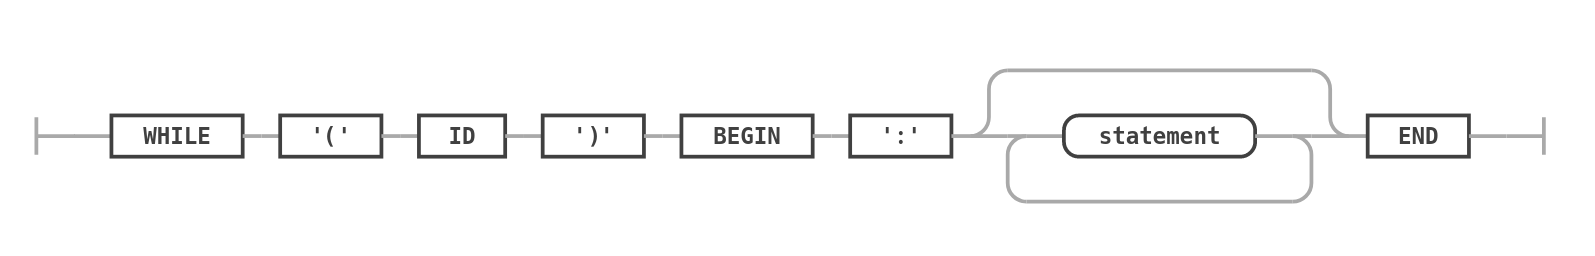
\includegraphics[width=14cm]{content/pictures/while.png}
	\caption{Die Grammatikregel für eine while-Schleife}
	\label{pic:WhileRegelWhile}
\end{figure}

Wie ein Statement definiert wird, ist in \cref{pic:WhileRegelStatement} zu erkennen. Als Statement werden viele unterschiedliche Konzepte bezeichnet: ein \textbf{succ} und \textbf{pred} sind statements oder auch \textbf{while} und \textbf{loop}. Aus den beiden Diagrammen lässt sich schließen, dass die Sprache auch Schleifen innerhalb von while-Schleifen erlaubt, was auch der Fall ist. 

\begin{figure}[h!]
	%\includegraphics[width=1\textwidth]{content/pictures/LoRaWAN-OSI.JPG}
	\centering
	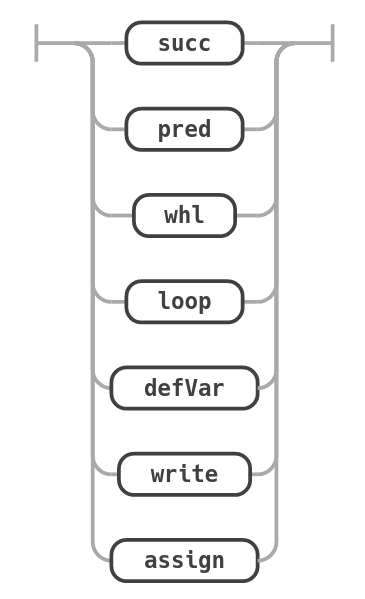
\includegraphics[width=4cm]{content/pictures/statement.png}
	\caption{Die Grammatikregel für ein Statement}
	%	\source{\cite[S. 5]{SemtechCorporation.2020}}
	\label{pic:WhileRegelStatement}
\end{figure}

Wenn ein Programm einer Menge von Grammatikregeln entspricht, bedeutet das nicht zwingend, dass der Programmcode fehlerfrei ist. Es existieren Fehleingaben, welche nur schwer durch Grammatikregeln erkannt werden können. Beispielsweise erlaubt die oben gezeigte Grammatik eine Wertzuweisung ohne vorauszusetzen, dass die entsprechende Variable zuvor definiert wurde. Um solche Fehler zu erkennen wird eine sogenannte semantische Analyse durchgeführt. Dieses Thema wird in \cref{chap:semantic} behandelt.




\chapter{Lexer und Parser}

Lexer und Parser generiert mit ANTLR\\
Visitor\\
Generierte Klassen\\

\chapter{Semantische Analyse} \label{chap:semantic}

Funktionsweise der Prüfungen (Ort und wie geprüft wird)\\

\chapter{Codegenerierung}

Aufgabe des Codegenerators \\
Mit Java ASM\\
Generierung von ausführbarem Bytecode für JVM\\
\section{Java ASM}
Bei ASM handelt es sich um ein aktuelles Framework zur Manipulation und Analyse von Java Bytecode. Es ermöglicht die Modifikation bestehender und das Erstellen neuer Klassen direkt in Bytecode. Dieses Framework wird unter anderem im Groovy und Kotlin Compiler eingesetzt, weshalb sich entschieden wurde ASM für diese Arbeit zu nutzen.

\\
//Reverseengineering von selbstgeschriebenen Java Code
\\
//Generierung von Java Maschinencode

\section{Abbildung von WHILE auf Java}
Bevor Bytecode erzeugt werden kann, muss überlegt werden, wie die Konzepte aus der Sprache WHILE in Java umzusetzen wären. Anschließend können die Javakonzepte in Java-Bytecode umgesetzt werden. Beispielsweise existiert in der Programmiersprache WHILE kein Konzept, welches Klassen entspricht. Aus diesem Grund entspricht ein WHILE-Programm immer einer einzigen Javaklasse und wie Klassen mithilfe von ASM erzeugt werden, wurde in \cref{subsec:asm-classwriter} bereits vorgestellt.

\subsection{Funktionen}
WHILE erlaubt es Statements innerhalb aber auch außerhalb von Funktionen zu schreiben, während in Java jede Anweisung innerhalb einer Methode stehen muss. Die Anweisungen in der Main-Methode werden beim Programmstart von oben nach unten ausgeführt. Um nun ein WHILE Programm auf Java abzubilden, wurde entschieden jedes Statement, welches sich außerhalb einer Funktion befindet, in der Java Main-Methode umzusetzen. 

Funktionen in WHILE und Java sind sich sehr ähnlich, weshalb While-Funktionen direkt auf Java-Methoden abgebildet werden können. Jeder Parameter einer Funktion und auch die Rückgabe ist immer vom Typ \enquote{BigInteger} Es wurde entschieden, jede Methode als \enquote{STATIC} zu deklarieren, da dies Funktionsaufrufe in der Main-Methode simplifiziert. In \cref{lst:asm-whileAufJava} ist zu sehen, wie eine solche Abbildung exemplarisch aussieht.

\begin{lstlisting}[language=Java, caption=Abbildung von While Funktionen auf Java Funktionen, label={lst:asm-whileAufJava}]
// Programm in WHILE
var r0 := 5;

def addTwo(s1) BEGIN:
	var retVal := s1;
	succ(retVal);
	succ(retVal);
	return retVal;
end

var r1 = addTwo(r0);

// Programm in Java
class Programm{
	
	// succ, pred und read sind hier definiert

	public static BigInteger addTwo(Biginteger s1) {
		BigInteger retVal = s1;
		Programm.succ(retVal);
		Programm.succ(retVal);
		return retVal;
	}

	public static void main(String args[]) {
		BigInteger r0 = new BigInteger("5");
		BigInteger r1 = Programm.addTwo(r0);
	}

}

\end{lstlisting}

\subsection{Schleifen und Variablen Definitionen}
In der Programmiersprache WHILE existieren neben den bekannten While-Schleifen auch Loop-Schleifen, für die es kein Java-Äquivalent gibt. Da der Unterschied zwischen While-Schleife und Loop-Schleife nur sehr gering ist, wird die Loop-Schleife als eine While-Schleife umgesetzt, welche die Variable im Schleifenkopf automatisch bei jedem Durchgang erniedrigt. In der Welt von ASM existieren keine Unterschiede zwischen while-, loop-, oder Do-While-Schleifen. Sie werden alle durch Vergleiche und GOTO-Anweisungen umgesetzt.

\subsection{PRED, SUCC, READ, WRITE}
Die WHILE Sprachkonzepte \enquote{PRED}, \enquote{SUCC} und \enquote{READ} verhalten sich wie in die Sprache eingebaute Funktionen. Sie sind fest definiert und die Implementation besteht aus mehreren Zeilen Java-Code, da Überprüfungen stattfinden. Es bietet sich daher an, diese Operationen tatsächlich als Methoden umzusetzen. Dazu wurde zunächst jede der genannten Funktionen als Java Programm geschrieben und anschließend mithilfe von ASMifer (\cref{subsec:asmifer}) der erzeugte ASM Code generiert, welcher zuletzt in den Codegenerator eingesetzt wurde. Diese Methoden werden bei jedem Kompiliervorgang dem Programm hinzugefügt, wie in \cref{lst:asm-whileAufJava} zu sehen ist.

Ausschließlich das Sprachkonstrukt \enquote{WRITE} wurde anders umgesetzt. Ein WRITE wird direkt in ein System.out.println() abgebildet.

\chapter{IDE-Integration}

VS-Code Language Server\\

\chapter{Anleitungen}

\section{Die \acs{vsc} Erweiterung installieren}

\section{Den Compiler verwenden}

\section{Den Compiler kompilieren}

\section{Den Compiler erweitern} 
\subsection{Grammatik anpassen}

\subsection{Semantische Überprüfung implementieren}

\subsection{Codegenerierung}

% Schalgwortverzeichnis (Index)
%\printindex

% Literaturverzeichnis
\singlespacing
%\nocite{*}
%\bibliographystyle{myIEEE.bst}
%\bibliography{IEEEabrv, bibtex}
\printbibliography[title=Literaturverzeichnis, heading=bibintoc]


%Zurücksetzen \chaptermark
\let\chaptermark\oldchaptermark

% Hier können Anhaenge angefuegt werden
\begin{appendices}
\appendixchapter{Die Grammatik der Sprache}
\monthlyreport{Teil 1}{content/attachments/While-1.pdf}
\monthlyreport{Teil 2}{content/attachments/While-2.pdf}
\end{appendices}

\end{document} 
